% Made up for the tikra benchmark.
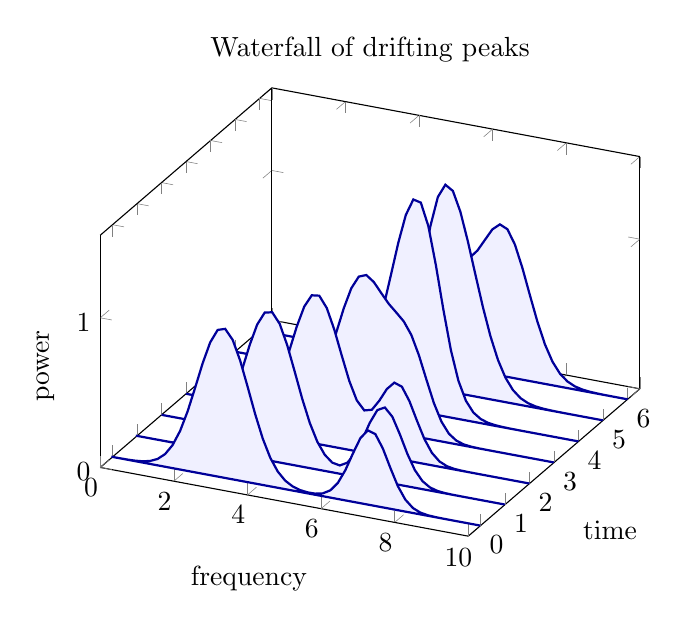
\begin{tikzpicture}
\begin{axis}[view={25}{35}, xlabel={frequency}, ylabel={time}, zlabel={power},
    title={Waterfall of drifting peaks}, ymin=-0.5, ymax=6.5, zmin=0, ytick={0,...,6}]
  \foreach \k in {6,5,...,0} {
    \addplot3[fill=blue!6, draw=blue!60!black, thick, samples=50, domain=0:10, samples y=0]
      (x, \k, {exp(-(x-3-0.6*\k)^2) + 0.5*exp(-(x-7+0.3*\k)^2/0.5)}) \closedcycle;
  }
\end{axis}
\end{tikzpicture}
